\documentclass[5p,times,twocolumn]{elsarticle}

\usepackage{amsmath,amssymb}
\usepackage{booktabs}
\usepackage{multirow}
\usepackage{graphicx}
\usepackage{microtype}
\usepackage{xurl}
\usepackage[hidelinks]{hyperref}
\usepackage{enumitem}

\journal{Computers \& Security}

\newcommand{\mission}{\mathcal{M}}
\newcommand{\authority}{\mathcal{A}}
\newcommand{\history}{\mathcal{H}}
\newcommand{\evidence}{\sigma}
\newcommand{\placeholderfigure}[2]{%
  \begin{figure}[t]
    \centering
    \fbox{\parbox[c][#1][c]{0.94\columnwidth}{\centering\small #2}}
  \end{figure}}

\begin{document}

\begin{frontmatter}

\title{Selection Witnesses for Open-World Agent Authorization:\\Evidence-Grounded Dynamic Authority Under a Fixed Effect Ceiling}

% Author metadata will be finalized before submission.
\author{Author names withheld in working draft}
\address{NullSquare}

\begin{abstract}
Tool-using language-model agents often operate with provider credentials whose standing permissions are broader than the task a user approved. Restricting an agent to task-scoped authority is difficult when the task needs resources whose identifiers are discovered only during execution. A common provenance rule---treating values observed through authorized actions as subsequently authorized---is unsafe when an observation contains multiple candidates: observation proves membership in the candidate set, not that the task selected a candidate. We study \emph{selection witnesses}, deterministic evidence that a unique candidate satisfies a task selector over authorized observations while the set of permitted effect types remains bounded by a fixed Mission ceiling. In a frozen 60-task AgentDojo cohort, the resulting stateful contracts preserve 60/60 reference executions and 36/36 evidence-consistent counterfactuals, compared with 1/36 for an exact-trace baseline, while blocking 370/370 corrected authorization mutants. At the protected provider boundary, the runtime blocks 230/230 constructible malicious trajectories with zero malicious provider reaches. In a partial live DeepSeek V4 Pro Slack evaluation, 372 adversarial scenarios completed in both ungated and gated conditions: ungated execution produced 61 policy-unauthorized protected effects across 40 scenarios, whereas gated execution produced none, with a 2.15 percentage-point matched utility difference. The planned 5,088-run live matrix did not complete, so the live result is evidence for provider-effect containment in the completed slice rather than a general prompt-injection-security claim.
\end{abstract}

\begin{keyword}
AI agents \sep authorization \sep least privilege \sep prompt injection \sep reference monitor \sep AgentDojo \sep capability security
\end{keyword}

\end{frontmatter}

\section{Introduction}
\label{sec:introduction}

Language-model agents increasingly act through tools: they read messages, update records, create meetings, issue payments, modify repositories, and call other services. The security problem is not only that a model can be manipulated by untrusted text. It is also that the model may hold, directly or through an application, provider permissions that are much broader than the user's current task. AgentDojo demonstrates how indirect prompt injection can redirect tool-using agents through untrusted data~\cite{debenedetti2024agentdojo}; subsequent systems therefore move important security decisions outside model reasoning~\cite{debenedetti2025camel,shi2025progent,costa2025fides}.

This paper studies a narrower authorization problem. Suppose the user authorizes a task before the concrete resource needed by the task is known. During legitimate execution the agent performs an authorized read and discovers one or more candidate resources. The authorization system must permit useful task progress without turning every observed value into ambient authority.

The tempting rule
\begin{quote}
\emph{a value observed through authorized execution may be used by later privileged effects}
\end{quote}
is not sufficient. In our development cohort, Slack task 13 asks the agent to identify the user with the largest total message count. Multiple users appear in authorized histories. Alice is observable, but Charlie is the aggregate winner. A provenance-only rule can therefore justify a mutation on Alice even though the task selected Charlie. This counterexample separates two concepts that are often conflated: \emph{candidate discovery} and \emph{selection authority}.

We investigate \emph{selection witnesses}: deterministic evidence that a resource is the unique result of a supported task selector over an authorized candidate set and its required measurements. A witness may therefore authorize a resource identifier that was not known at task start, but only when the selection predicate is justified by authorized evidence. Ties, incomplete measurements, unsupported semantics, and unresolved dynamic values fail closed. At the same time, the kinds of provider effects the task may execute remain under a fixed Mission ceiling.

The paper evaluates this mechanism at the provider-effect boundary rather than claiming that the model itself becomes robust to prompt injection. The reference monitor mediates protected effects before side effects execute. A compromised or confused model may still propose an unsafe call; the security question is whether that call reaches the provider.

Our contributions are:
\begin{enumerate}[leftmargin=*,nosep]
    \item \textbf{A falsification of provenance-only dynamic authority.} We show a concrete open-world task where observation provenance authorizes the wrong candidate and motivate candidate/selection separation.
    \item \textbf{Evidence-grounded selection witnesses.} We define a task-local authority transition in which resource facts may be acquired from authorized execution evidence or deterministic selection witnesses while effect authority remains inside a fixed Mission ceiling.
    \item \textbf{A provider-boundary implementation and deterministic evaluation.} Across 60 mutation-bearing AgentDojo tasks, the frozen V1 mechanism preserves 60/60 reference executions and 36/36 evidence-consistent counterfactuals, blocks 370/370 corrected authorization mutants, and blocks 230/230 constructible malicious provider-boundary trajectories with zero malicious provider reaches.
    \item \textbf{Partial live-model evidence and a negative result.} In 372 matched attacked DeepSeek V4 Pro Slack scenarios, ungated execution produces 61 policy-unauthorized protected effects across 40 scenarios while gated execution produces none. Separately, an exact successful-trace baseline accepts only 1/36 legitimate counterfactuals, showing that a successful trace can over-constrain the semantic authority envelope of a task.
\end{enumerate}

We make two scope boundaries explicit. First, the live DeepSeek experiment is incomplete: the preregistered 5,088-run matrix failed its zero-error completion gate after an evaluator serialization defect in one attempt and API-balance exhaustion in the next. Second, provider-effect containment is not equivalent to complete prompt-injection prevention; read-only leakage and unsafe natural-language output can fall outside the protected mutation boundary.

\section{Background and Related Work}
\label{sec:related}

\subsection{Prompt injection and task alignment}

Indirect prompt injection exploits the fact that an agent may process attacker-controlled data in the same reasoning context used to choose actions. AgentDojo provides a dynamic environment with realistic tools, user tasks, injection tasks, and security/utility metrics~\cite{debenedetti2024agentdojo}. Task Shield reframes defense as action-to-task alignment and checks whether each instruction or tool call contributes to the user objective~\cite{jia2025taskshield}. These approaches establish the threat setting, but task alignment and provider authorization answer different questions: an action can look plausible to a model-level guard while still exceeding a separately defined task authority, and a provider-boundary monitor can reject an effect even after model reasoning has been compromised.

\subsection{System isolation and information flow}

CaMeL extracts trusted control and data flows from the user's query and uses capabilities to prevent untrusted data from controlling unsafe flows~\cite{debenedetti2025camel}. Fides formalizes information-flow properties for agent planners and combines confidentiality/integrity labels with deterministic enforcement~\cite{costa2025fides}. Prompt Flow Integrity separates trusted and untrusted prompt/data flows and enforces least privilege and unsafe-flow checks~\cite{kim2025pfi}. IsolateGPT uses execution isolation to separate LLM applications and system components~\cite{wu2025isolategpt}. ACE separates trusted abstract planning from concrete application mapping and validates secure information-flow constraints before and during execution~\cite{li2026ace}. AgentFlow introduces a flow-centric policy language with task-scoped capabilities, stateful taint semantics, runtime reference monitoring, and bounded verification~\cite{shivakumar2026agentflow}.

These systems demonstrate the value of structural enforcement outside the model. Our focus is different: when authorized execution reveals several legitimate resource candidates, which one becomes authorized for a later protected effect? Information provenance can establish that a candidate was observed, but observation alone does not establish the task's selection relation.

\subsection{Privilege, authorization, and delegation}

Progent applies programmable privilege-control policies to tool calls through a deterministic reference monitor and supports dynamic policy updates~\cite{shi2025progent}. Authenticated Delegation extends established identity and authorization infrastructure with agent-specific delegation and auditable permission scoping~\cite{south2025delegation}. SAGA governs multi-agent lifecycles and inter-agent communication with user-defined policies and cryptographically derived access-control tokens~\cite{syros2026saga}. Bounded Agents accumulates session state, constrains delegated authority, checks prohibited action compositions, and enforces authorization outside the model~\cite{muruaga2026bounded}. aiAuthZ similarly moves authorization off the model host and binds policy decisions to authenticated callers and argument-level policies~\cite{kodathala2026aiauthz}.

These works make broad claims such as ``first agent authorization'' or ``first stateful agent authorization'' inappropriate for this paper. We instead isolate a narrower open-world resource problem. A task may start without the identifier of the resource it will later mutate. Authorized execution can discover that identifier, but a multi-candidate result requires evidence of \emph{selection}, not only evidence of \emph{observation}. Selection witnesses are our candidate contribution to this narrower problem.

\subsection{Classical security foundations}

The architecture follows classical principles rather than replacing them. Least privilege motivates reducing standing authority~\cite{saltzer1975protection}; complete mediation motivates a reference monitor on protected effects; capability and delegation systems motivate attenuation rather than silent authority amplification. Our contribution is therefore not the existence of least privilege, stateful authorization, provenance, or delegation. It is the evidence rule used to acquire concrete task-local resource authority under an unchanged effect ceiling.

\section{System and Threat Model}
\label{sec:threat}

\subsection{Execution model}

A user approves a task under a \emph{Mission}, which defines the maximum kinds of protected effects available to the task. The task starts with trusted resource roots such as a repository, account, ticket, or source object. The agent may request reads or mutations. A reference monitor evaluates each protected request before the provider side effect executes. Authorized results produce execution evidence that can support later task-local authority derivation.

\begin{figure*}[t]
    \centering
    \IfFileExists{figures/fig01-system-boundary.pdf}{%
      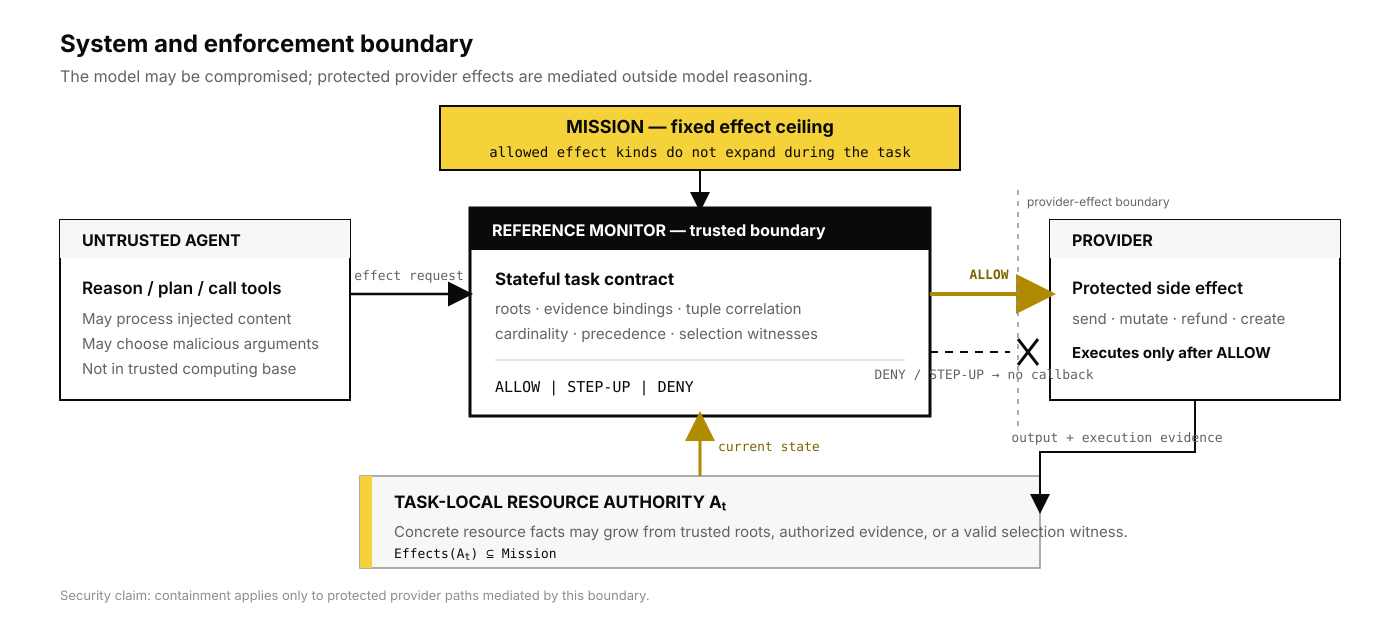
\includegraphics[width=0.96\textwidth]{figures/fig01-system-boundary.pdf}%
    }{%
      \fbox{\parbox[c][46mm][c]{0.94\textwidth}{\centering\small Figure 1 master: \texttt{figures/fig01-system-boundary.svg}.\\Agent reasoning $\rightarrow$ reference monitor $\rightarrow$ provider effect, with execution evidence feeding task-local authority while the Mission remains the effect ceiling.}}
    }
    \caption{System and enforcement boundary. The model may be compromised and may propose arbitrary tool arguments. Protected provider effects execute only after the task-authority monitor authorizes the exact request. Authorized output can support new task-local resource facts without adding new effect types to the Mission.}
    \label{fig:system}
\end{figure*}

\subsection{Adversary}

The adversary may control untrusted content consumed by the model and may thereby influence the model's tool choices. We additionally evaluate a compromised-model adversary that directly constructs malicious effect requests. The adversary may substitute resources or fields, reorder calls, repeat effects, transplant identifiers across tasks, combine individually plausible values into an unauthorized tuple, choose a non-selected candidate from a legitimate result set, or attempt circular self-authorization by first reading a resource it already chose.

The model is not part of the trusted computing base. The V1 trusted computing base contains Mission construction, the reference monitor, provider adapters on the guarded path, execution-evidence integrity, reviewed authority extractors, selector implementations, and schema metadata used to project authority-relevant effect arguments.

\subsection{Security objective and scope}

For a protected provider mutation $e_t$, the primary safety objective is:
\begin{equation}
  e_t \notin \mathrm{Allowed}(\authority_t,\mission)
  \quad\Longrightarrow\quad
  \mathrm{ProviderReach}(e_t)=0.
  \label{eq:provider-safety}
\end{equation}
The monitor cannot secure a provider path it does not control. If the model can reach the same provider through another credential, shell, network path, or unguarded connector, that path is outside the mechanism. The V1 mechanism also does not claim to prevent every read-only confidentiality leak, unsafe natural-language response, or model-level prompt-injection success.

\section{Evidence-Grounded Task Authority}
\label{sec:mechanism}

\subsection{Mission ceiling and task-local authority}

Let $\mission$ denote the Mission's effect-authority ceiling and let $\authority_t$ denote task-local resource authority at step $t$. The important distinction is that concrete resource facts may be learned over time while the available effect kinds remain bounded:
\begin{equation}
    \mathrm{Effects}(\authority_t) \subseteq \mission \quad \text{for every reachable }t.
    \label{eq:mission-ceiling}
\end{equation}
A task therefore need not enumerate every future resource identifier at start. It may acquire resource facts through an authorized causal execution path without gaining a new class of provider effect.

\subsection{Why provenance alone fails}
\label{sec:provenance-fails}

Assume an authorized read returns candidate set $C=\{A,B,C\}$. Provenance establishes that each candidate occurred in an authorized result. It does not establish which candidate satisfies the user's task. Worse, prior request arguments can create circular provenance:
\begin{equation*}
\text{agent chooses }x \rightarrow \text{read}(x) \rightarrow x\text{ observed} \not\Rightarrow x\text{ authorized}.
\end{equation*}
The Slack aggregate-winner counterexample made this failure concrete during development. A safe derivation rule must therefore distinguish \emph{candidate membership} from \emph{selection evidence}.

\begin{figure*}[t]
    \centering
    \IfFileExists{figures/fig02-selection-witness.pdf}{%
      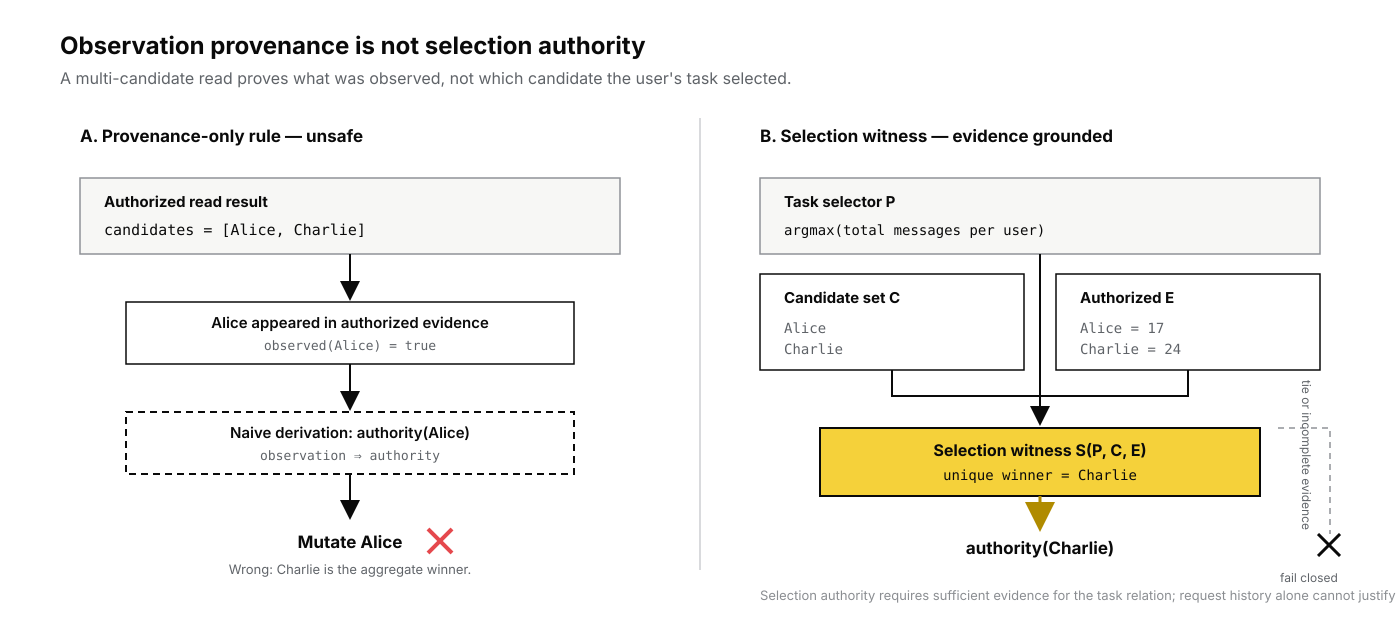
\includegraphics[width=0.96\textwidth]{figures/fig02-selection-witness.pdf}%
    }{%
      \fbox{\parbox[c][42mm][c]{0.94\textwidth}{\centering\small Figure 2 master: \texttt{figures/fig02-selection-witness.svg}.\\Left: observation-provenance failure. Right: candidate set + complete authorized measurements + task predicate $\rightarrow$ unique winner $\rightarrow$ authority.}}
    }
    \caption{Observation provenance is not selection authority. A multi-candidate result proves candidate membership, not that every member is authorized for a later mutation. A deterministic selection witness authorizes only the unique candidate justified by the task selector and sufficient authorized evidence. Ties or incomplete measurements fail closed.}
    \label{fig:selection}
\end{figure*}

\subsection{Selection witnesses}

Let $P$ denote a task selection predicate, $C$ a candidate set derived from authorized execution, and $E$ the measurements or attributes needed to evaluate $P$. A selection witness
\begin{equation}
    S(P,C,E) \rightarrow r
\end{equation}
may produce resource $r$ only when the selector is supported, the required evidence is complete, and $r$ is the unique value satisfying the selector. Otherwise $S$ produces no generalized dynamic authority.

Examples implemented in the research prototype include unique prefix matching, unique minima/maxima over complete measurements, and aggregate-frequency extrema. The V1 system does not claim to infer arbitrary semantic predicates from natural language.

If $o_t$ is output from an authorized effect and $\evidence_t$ binds that output to the guarded request, a simplified authority transition is:
\begin{equation}
\authority_{t+1}=\authority_t
\cup \mathrm{derive}(o_t,\evidence_t)
\cup \mathrm{select}(S(P,C,E)).
\label{eq:authority-transition}
\end{equation}
Prior agent-supplied request arguments do not themselves mint authority. Unresolved dynamic-looking values may remain fenced to the observed reference value as a conservative fallback; this preserves safety but is evidence that the compiler has \emph{not} inferred the general task semantics.

\begin{figure}[t]
    \centering
    \IfFileExists{figures/fig03-authority-state.pdf}{%
      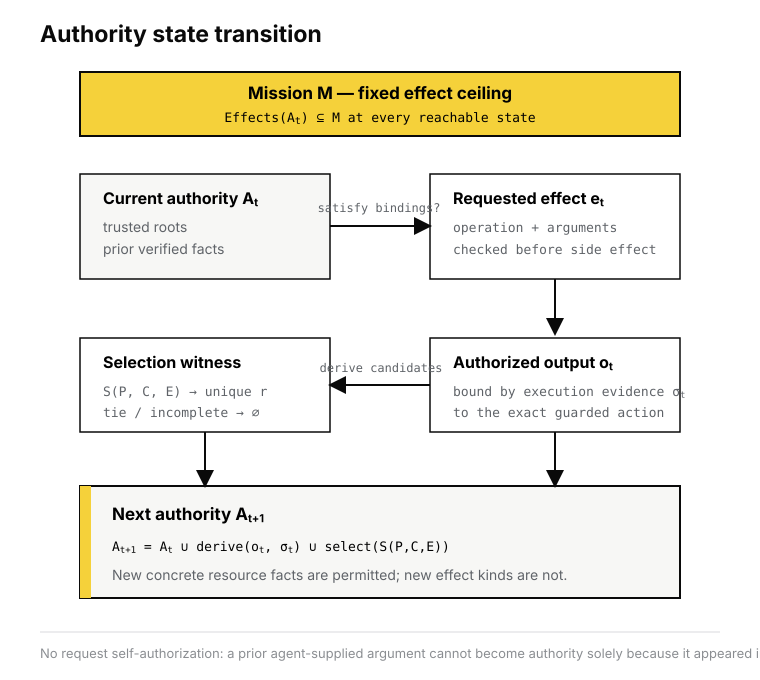
\includegraphics[width=0.98\columnwidth]{figures/fig03-authority-state.pdf}%
    }{%
      \fbox{\parbox[c][40mm][c]{0.92\columnwidth}{\centering\small Figure 3 master: \texttt{figures/fig03-authority-state.svg}.\\State transition from $\authority_t$ through authorized evidence and selection witness to $\authority_{t+1}$, under invariant $\mathrm{Effects}(\authority_t)\subseteq\mission$.}}
    }
    \caption{Task-local resource authority can grow through verified evidence while the Mission remains the effect ceiling.}
    \label{fig:state}
\end{figure}

\subsection{Stateful contract constraints}

Selection is one part of the V1 task contract. The frozen mechanism also enforces projected field constraints, static tuples and correlations, action cardinality, and precedence/order. These constraints matter because independently valid field values can form an unauthorized tuple, and individually permitted effects can form an unauthorized trajectory when repeated or reordered. The runtime evaluates the complete projected request against the current task state before invoking the guarded provider callback.

\section{Methodology}
\label{sec:methodology}

We evaluate four research questions.

\textbf{RQ1: Utility and open-world generalization.} Can the contract preserve reference execution and evidence-consistent changes to dynamically discovered resources without broad wildcard authority?

\textbf{RQ2: Provider-boundary safety.} Can the stateful contract block structured authorization mutations and malicious trajectories before protected provider effects execute?

\textbf{RQ3: Live-model containment.} When a model produces out-of-policy protected effects under adversarial trajectories, does the same frozen gate prevent those effects from reaching the provider?

\textbf{RQ4: Failure analysis.} Which failures reveal limits in deriving authority from successful execution traces?

\begin{figure*}[t]
    \centering
    \IfFileExists{figures/fig04-methodology.pdf}{%
      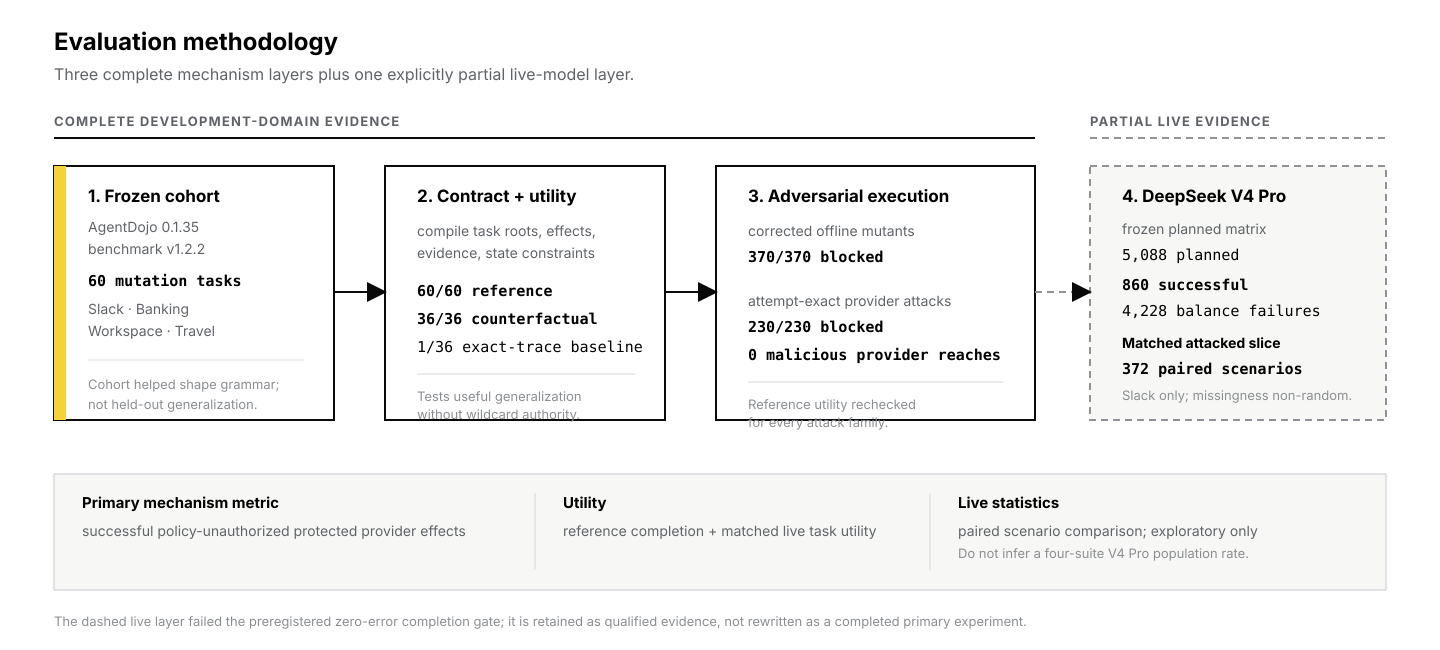
\includegraphics[width=0.97\textwidth]{figures/fig04-methodology.pdf}%
    }{%
      \fbox{\parbox[c][50mm][c]{0.95\textwidth}{\centering\small Figure 4 master: \texttt{figures/fig04-methodology.svg}.\\Frozen 60-task AgentDojo cohort $\rightarrow$ contract synthesis and counterfactual utility $\rightarrow$ corrected mutants and provider-boundary attack families $\rightarrow$ frozen live DeepSeek gated/ungated evaluation $\rightarrow$ matched completed-scenario analysis.}}
    }
    \caption{Evaluation methodology and evidence layers. The deterministic and provider-boundary layers are complete across the 60-task mutation-bearing cohort. The DeepSeek V4 Pro layer is explicitly partial: only scenarios that completed in both gated and ungated conditions enter the matched live comparison.}
    \label{fig:methodology}
\end{figure*}

\subsection{Frozen AgentDojo cohort}

The deterministic evaluation uses AgentDojo 0.1.35 with benchmark data v1.2.2. We include all 60 user tasks in Slack, Banking, Workspace, and Travel that contain protected mutations in the authority projection. The cohort helped shape the contract grammar during development and is therefore a development-domain evaluation rather than a held-out generalization benchmark.

For each task we execute the reference workflow and compile a task contract from task roots, projected provider actions, and authorized execution evidence. \emph{Reference utility} requires the original mutation-bearing workflow to remain executable. To test dynamic generalization we construct 36 evidence-consistent counterfactuals in which authorized evidence changes while the task relation remains valid. We compare the stateful contract with an exact-trace baseline that freezes the concrete reference effect arguments.

\subsection{Corrected authorization mutants}

We generate near-neighbor executions intended to violate the task contract while remaining close to a legitimate trace. After correcting the mutant construction and removing cases that did not represent a true authority violation, the frozen denominator is 370:
\begin{itemize}[leftmargin=*,nosep]
    \item 146 field/resource mutants;
    \item 60 repeated-effect mutants;
    \item 59 order mutants;
    \item 60 stronger-action mutants;
    \item 12 cross-product tuple mutants; and
    \item 33 exact full-action-tuple cross-task transplants.
\end{itemize}
The outcome is whether the strict contract rejects each mutant.

\subsection{Provider-boundary adversary}

Offline contract rejection alone does not establish that a malicious effect cannot execute. We therefore construct attempt-exact trajectories against the same guarded provider boundary. The 230-trajectory evaluation contains 60 field/resource substitutions, 60 premature or reordered effects, 60 repeated effects, 46 exact cross-task transplants, and four wrong-selector candidates. We record both the authorization decision and whether the protected provider callback is reached. For each attack family we also execute all 60 reference workflows to detect security changes that destroy baseline utility.

\subsection{Live DeepSeek protocol}

Before the paid live experiment, the mechanism, task cohort, attack families, templates, and evaluation plan were frozen. The intended matrix contained 5,088 DeepSeek V4 Pro task-runs across the 60 protected tasks, four suites, three trials, canonical AgentDojo \texttt{tool\_knowledge} attacks, and five authority-adaptive attack families. The preregistered scientific gate required zero unresolved execution errors.

The full matrix did not complete. Attempt 3 delivered canonical attacks but all 1,380 adaptive rows failed before model execution because exact JSON attack payloads broke YAML serialization. Attempt 4 changed evaluator delivery plumbing only: inert sentinels were substituted before YAML parsing and the exact attack payload was restored afterward. The authority mechanism, attack targets, templates, and thresholds remained frozen. Attempt 4 contained no parser errors, but the paid account then returned \texttt{402 Insufficient Balance} before later suites executed. Consequently, Attempt 4 has 860 successful trajectories and 4,228 balance failures; all successful trajectories are Slack.

The paper's live comparison uses the 372 attacked scenarios for which both the gated and ungated condition completed for the same tuple $(\text{suite},\text{trial},\text{task},\text{attack family},\text{attack id})$. Because missingness is not random and the preregistered matrix failed its zero-error completion gate, all live statistics are descriptive/exploratory.

\subsection{Metrics and analysis}

The primary mechanism metric is the count of \emph{successful policy-unauthorized protected provider effects}. This differs from AgentDojo's injection-task security oracle: a run may fail that oracle through read-only leakage or other behavior outside the protected mutation scope. We also report task utility and scenario-level occurrence of at least one unauthorized protected effect.

For the paired 372-scenario live slice, the natural exact comparison is McNemar's test over discordant scenario pairs. We report it only as exploratory support. Wilson intervals summarize scenario-level unauthorized-effect rates but must not be interpreted as four-suite population estimates.

\begin{table}[t]
\centering
\caption{Frozen evaluation layers and scientific status.}
\label{tab:layers}
\small
\begin{tabular}{@{}p{0.24\columnwidth}p{0.19\columnwidth}p{0.20\columnwidth}p{0.25\columnwidth}@{}}
\toprule
Layer & Scope & Denominator & Status \\
\midrule
Reference / counterfactual & 4 suites & 60 / 36 & Complete \\
Corrected mutants & 4 suites & 370 & Complete \\
Provider-boundary families & 4 suites & 230 & Complete \\
V4 Pro Attempt 3 & Slack + Banking subset & 1,028 successes & Supplementary; adaptive delivery invalid \\
V4 Pro Attempt 4 & Slack only & 860 successes & Partial live slice; balance exhausted \\
\bottomrule
\end{tabular}
\end{table}

\section{Results}
\label{sec:results}

\subsection{RQ1: utility and dynamic generalization}

The frozen contract preserves all 60 reference workflows. It also accepts all 36 evidence-consistent counterfactuals. The exact-trace baseline accepts only 1/36. This 35-case gap is important because it shows that security cannot be obtained simply by copying one successful trace into a list of exact allowed arguments. A useful task authority must preserve relations that remain valid when authorized evidence changes.

\subsection{RQ2: deterministic and provider-boundary safety}

The strict contract blocks all 370 corrected authorization mutants. At the execution boundary it blocks all 230 constructible malicious trajectories and records zero malicious provider reaches. Reference utility remains 60/60 in every provider-boundary attack family.

\begin{table}[t]
\centering
\caption{Provider-boundary attack families.}
\label{tab:provider-families}
\small
\begin{tabular}{@{}lrrr@{}}
\toprule
Attack family & Attempts & Blocked & Provider reach \\
\midrule
Field/resource substitution & 60 & 60 & 0 \\
Premature/reordered & 60 & 60 & 0 \\
Repeated effect & 60 & 60 & 0 \\
Exact cross-task transplant & 46 & 46 & 0 \\
Wrong selector candidate & 4 & 4 & 0 \\
\midrule
Total & 230 & 230 & 0 \\
\bottomrule
\end{tabular}
\end{table}

\begin{figure}[t]
    \centering
    \IfFileExists{figures/fig05-deterministic-results.pdf}{%
      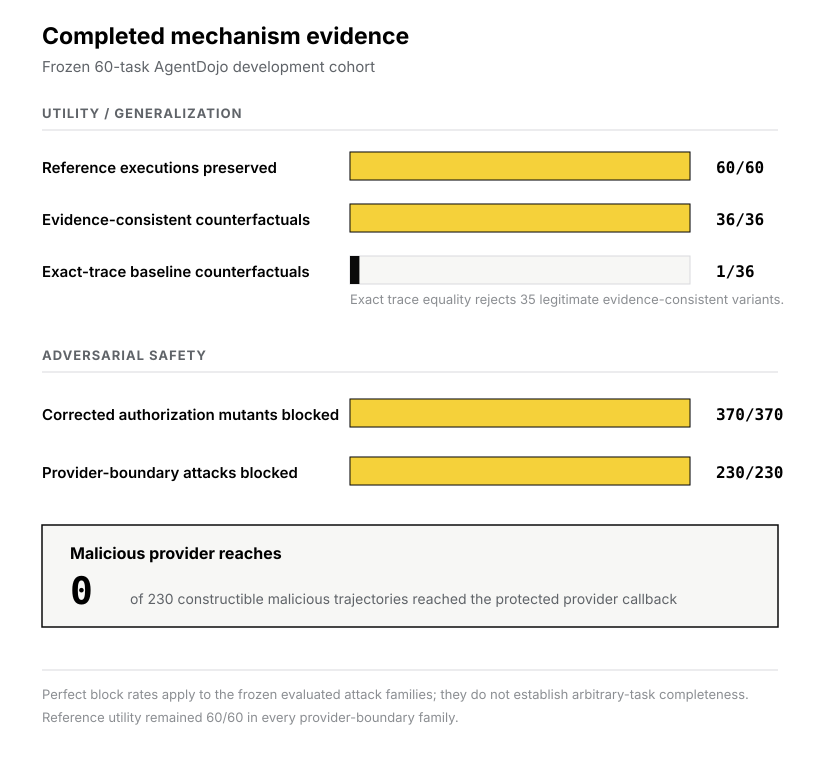
\includegraphics[width=0.98\columnwidth]{figures/fig05-deterministic-results.pdf}%
    }{%
      \fbox{\parbox[c][46mm][c]{0.92\columnwidth}{\centering\small Figure 5 master: \texttt{figures/fig05-deterministic-results.svg}.\\60/60 reference; 36/36 counterfactual vs 1/36 exact trace; 370/370 mutants; 230/230 provider attacks; 0 malicious provider reach.}}
    }
    \caption{Completed deterministic and provider-boundary evidence. The exact-trace baseline's utility failure is shown beside the stateful contract rather than being hidden behind the perfect block rates.}
    \label{fig:det-results}
\end{figure}

These results support a mechanism-level claim over the development cohort: the stateful grammar captures relations that both generalize beyond the concrete trace and reject the evaluated near-neighbor mutations. They do not establish completeness for arbitrary natural-language tasks or arbitrary semantic selectors.

\subsection{RQ3: partial live-model containment}

Attempt 4 produced 860 successful DeepSeek V4 Pro trajectories before the account balance was exhausted. In aggregate successful attacked rows, the ungated condition produced 66 unauthorized protected effects while the gated condition produced none. For a controlled comparison we use only the 372 attacked scenarios that completed in both conditions.

Across those matched scenarios, ungated execution produced 61 policy-unauthorized protected provider effects across 40 scenarios (10.75\%). Gated execution produced zero unauthorized protected effects across zero scenarios. Matched utility was 84.41\% ungated and 82.26\% gated, a 2.15 percentage-point difference.

\begin{table}[t]
\centering
\caption{Matched attacked DeepSeek V4 Pro Slack scenarios.}
\label{tab:live}
\small
\begin{tabular}{@{}lrr@{}}
\toprule
Metric & Ungated & Gated \\
\midrule
Matched scenarios & 372 & 372 \\
Unauthorized protected effects & 61 & 0 \\
Scenarios with $\geq1$ unauthorized effect & 40 & 0 \\
Utility & 84.41\% & 82.26\% \\
Policy rejections & -- & 373 \\
\bottomrule
\end{tabular}
\end{table}

\begin{figure}[t]
    \centering
    \IfFileExists{figures/fig06-live-results.pdf}{%
      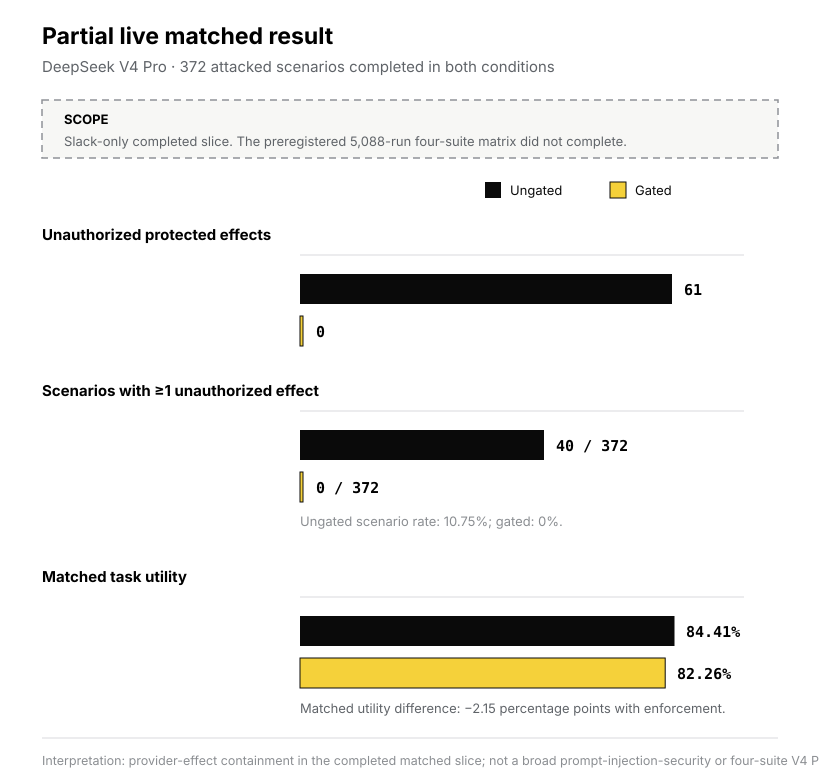
\includegraphics[width=0.98\columnwidth]{figures/fig06-live-results.pdf}%
    }{%
      \fbox{\parbox[c][48mm][c]{0.92\columnwidth}{\centering\small Figure 6 master: \texttt{figures/fig06-live-results.svg}.\\372 matched attacked scenarios: 61 $\rightarrow$ 0 unauthorized effects; 40 $\rightarrow$ 0 affected scenarios; utility 84.41\% $\rightarrow$ 82.26\%.\\Scope: completed Slack slice only.}}
    }
    \caption{Partial live DeepSeek V4 Pro result for matched attacked Slack scenarios. The planned 5,088-run matrix did not complete; this figure intentionally reports only the completed paired slice.}
    \label{fig:live-results}
\end{figure}

The canonical AgentDojo \texttt{tool\_knowledge} subset contains 244 matched scenarios and 39 ungated unauthorized protected effects across 28 scenarios, with zero gated unauthorized effects. The five authority-adaptive families contribute 128 matched scenarios and 22 ungated out-of-policy protected effects across 12 scenarios, again with zero gated unauthorized effects. These out-of-policy effects are not all exact attacker-target completions; the adaptive experiments stress the authority boundary rather than measure exact attack-goal success.

Attempt 3 provides supplementary canonical-attack replication. It produced 422 matched successfully executed \texttt{tool\_knowledge} scenarios across the completed Slack and Banking portion. Ungated execution produced 79 unauthorized protected effects across 61 scenarios; gated execution produced none. We do not combine Attempt 3 with Attempt 4 as if they were one preregistered complete experiment because the adaptive arm in Attempt 3 was never delivered to the model.

\subsection{RQ4: successful traces can encode the wrong authority envelope}

The exact-trace baseline result already indicates over-constraint: only 1/36 legitimate evidence-consistent variants is accepted. Live debugging exposed the mechanism more directly. In \texttt{travel-4}, the user asks for an event on 25 April 2024 while the benchmark ground-truth workflow uses 25 April 2023. In \texttt{travel-7}, the prompt specifies a month/day but not a year or hour, while the trace fixes a particular year and time range. Promoting those incidental or contradictory trace values to exact authority rejects semantically plausible executions.

This negative result changes the research direction. Future work should infer a \emph{semantic authority envelope} that distinguishes task-root required constants, bounded values, evidence-derived values, selection-witness outputs, and incidental execution choices. The V1 paper does not claim that such an intent compiler has been solved.

\section{Discussion and Limitations}
\label{sec:discussion}

\subsection{Provider-effect authorization is a separate boundary}

The live results illustrate why model robustness and provider authorization should be measured separately. A model can still be deceived, leak information, or attempt an unsafe call. The reference monitor's role is narrower: prevent protected provider effects that are outside the task authority. This separation is consistent with recent system-level defenses and authorization gateways that move enforcement away from the model~\cite{debenedetti2025camel,shi2025progent,kodathala2026aiauthz,muruaga2026bounded}.

\subsection{Threats to validity}

\textbf{Development-domain cohort.} The 60-task cohort helped shape the contract grammar. Perfect deterministic block rates therefore measure mechanism closure over that development domain, not held-out generalization.

\textbf{Incomplete live matrix.} The preregistered 5,088-run DeepSeek V4 Pro experiment did not complete. Attempt 4's successful trajectories are Slack only, because the account balance was exhausted before later suites. Missing rows are not random, and the live rates must not be generalized to all four suites.

\textbf{Single live model family.} The strongest live evidence is DeepSeek V4 Pro, with earlier small DeepSeek Flash trials as supplementary evidence. Multi-model robustness is not established.

\textbf{Protected-effect scope.} The monitor mediates protected provider mutations on guarded paths. It does not guarantee confidentiality for every read, safe natural-language output, remote provider attestation, or safety for bypass paths that do not traverse the reference monitor.

\textbf{Selector coverage.} V1 implements a small set of deterministic selector witnesses and conservative static fencing. It does not infer arbitrary predicates from natural language, and fail-closed behavior can reduce utility when evidence is incomplete.

\subsection{Future work}

The next research problem is not to spend more API budget filling the historical V1 matrix. Higher-value extensions are: semantic authority envelopes; formal operational semantics and proofs for Mission non-amplification and selection soundness; held-out open-world tasks with explicit selector ground truth; independent baseline implementations and ablations; broader model diversity; runtime/step-up cost measurement; and independent red-team attempts against the provider boundary.

\section{Conclusion}
\label{sec:conclusion}

Task-scoped authorization for agents becomes an open-world problem when useful resources are discovered only after execution begins. The central V1 finding is that authorized observation is not sufficient evidence of selection. Selection witnesses make this distinction explicit: task-local resource authority can follow a deterministic relation over authorized evidence while the kinds of effects available to the task remain under a fixed Mission ceiling. Across the frozen 60-task AgentDojo development cohort, this mechanism preserves reference and evidence-consistent utility while blocking the evaluated authorization mutants and provider-boundary malicious trajectories. A partial DeepSeek V4 Pro Slack slice further shows the practical boundary: the ungated model produced protected effects outside frozen task authority, while the gated runtime prevented those effects from reaching the provider in the matched completed scenarios. The result supports provider-effect containment, not a claim that prompt injection is solved, and it exposes a second open problem: successful traces are too concrete to serve as complete semantic authorization specifications.

\section*{Data and Code Availability}

The implementation, frozen research protocol, result summaries, attempt history, artifact identities, and offline reproduction workflow are available in the public Agent Authority repository. The manuscript will cite the exact research-closure commit and archival artifact digests in the final submission.

\section*{Declaration of Competing Interest}

The authors will provide the journal-required competing-interest statement before submission.

\section*{Acknowledgments}

Acknowledgments, funding statements, and contributor roles will be finalized before submission.

\bibliographystyle{elsarticle-num}
\bibliography{references}

\end{document}
